\documentclass[tikz]{standalone}
\begin{document}%
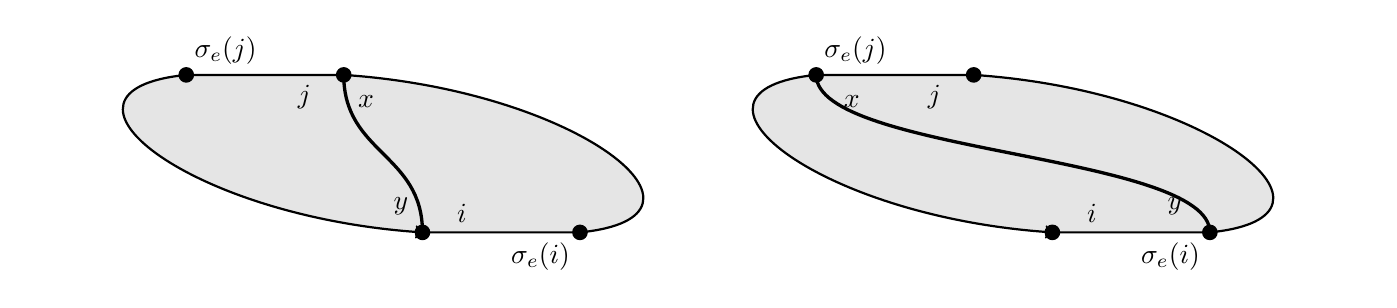
\begin{tikzpicture}[vert/.style={fill=black,circle,inner sep=2pt,outer sep=2pt}]

\coordinate (i0) at (0,0);
\coordinate (i1) at (2,0);

\coordinate (j0) at (-1,2);
\coordinate (j1) at (-3,2);

\fill[gray!20] (i0) -- (i1) .. controls +(2,0.2) and +(3,-0.2) .. (j0) -- (j1) .. controls +(-2,-0.2) and +(-3,0.2) .. (i0) -- cycle;

\draw[thick,->] (i0) -- node[above,near start] {$i$} node[below, near end] {$\sigma_e(i)$} (i1)
.. controls +(2,0.2) and +(3,-0.2) .. (j0) -- node[below,near start] {$j$} node[above, near end] {$\sigma_e(j)$} (j1) .. controls +(-2,-0.2) and +(-3,0.2) .. (i0);

\node[vert] at (i0) {};
\node[vert] at (i1) {};
\node[vert] at (j0) {};
\node[vert] at (j1) {};

\draw[very thick] (i1) .. controls +(0,1) and +(0,-1) .. node[left,very near start] {$y$} node[right,very near end] {$x$} (j1);

\begin{scope}[xshift=-8cm]
\coordinate (i0) at (0,0);
\coordinate (i1) at (2,0);

\coordinate (j0) at (-1,2);
\coordinate (j1) at (-3,2);

\fill[gray!20] (i0) -- (i1) .. controls +(2,0.2) and +(3,-0.2) .. (j0) -- (j1) .. controls +(-2,-0.2) and +(-3,0.2) .. (i0) -- cycle;

\draw[thick,->] (i0) -- node[above,near start] {$i$} node[below, near end] {$\sigma_e(i)$} (i1)
.. controls +(2,0.2) and +(3,-0.2) .. (j0) -- node[below,near start] {$j$} node[above, near end] {$\sigma_e(j)$} (j1) .. controls +(-2,-0.2) and +(-3,0.2) .. (i0);

\node[vert] at (i0) {};
\node[vert] at (i1) {};
\node[vert] at (j0) {};
\node[vert] at (j1) {};


\draw[very thick] (i0) .. controls +(0,1) and +(0,-1) .. node[left,very near start] {$y$} node[right,very near end] {$x$} (j0);
\end{scope}
\end{tikzpicture}%
\end{document}
